% Nicholas Arnold
% Steven Braeger
% CDA 5106
%
% Project Final Report
%
% We used the template from IEEE website, linked from
% http://www.ieee.org/conferences_events/conferences/publishing/templates.html	

\documentclass[conference]{IEEEtran}
\usepackage{algorithm}
\usepackage{algorithmic}
\usepackage{array}

% *** CITATION PACKAGES ***
%
%\usepackage{cite}
% cite.sty was written by Donald Arseneau
% V1.6 and later of IEEEtran pre-defines the format of the cite.sty package
% \cite{} output to follow that of IEEE. Loading the cite package will
% result in citation numbers being automatically sorted and properly
% "compressed/ranged". e.g., [1], [9], [2], [7], [5], [6] without using
% cite.sty will become [1], [2], [5]--[7], [9] using cite.sty. cite.sty's
% \cite will automatically add leading space, if needed. Use cite.sty's
% noadjust option (cite.sty V3.8 and later) if you want to turn this off.
% cite.sty is already installed on most LaTeX systems. Be sure and use
% version 4.0 (2003-05-27) and later if using hyperref.sty. cite.sty does
% not currently provide for hyperlinked citations.
% The latest version can be obtained at:
% http://www.ctan.org/tex-archive/macros/latex/contrib/cite/
% The documentation is contained in the cite.sty file itself.

% *** MATH PACKAGES ***
%
%\usepackage[cmex10]{amsmath}
% *** SPECIALIZED LIST PACKAGES ***
%
%\usepackage{algorithmic}
% algorithmic.sty was written by Peter Williams and Rogerio Brito.
% This package provides an algorithmic environment fo describing algorithms.
% You can use the algorithmic environment in-text or within a figure


% *** ALIGNMENT PACKAGES ***
%
%\usepackage{array}
%\usepackage{mdwmath}
%\usepackage{mdwtab}
%\usepackage{eqparbox}

% *** SUBFIGURE PACKAGES ***
%\usepackage[tight,footnotesize]{subfigure}

%\usepackage[caption=false]{caption}
%\usepackage[font=footnotesize]{subfig}
%\usepackage{fixltx2e}
%\usepackage{stfloats}
% stfloats.sty was written by Sigitas Tolusis. This package gives LaTeX2e
% the ability to do double column floats at the bottom of the page as well
% as the top. (e.g., "\begin{figure*}[!b]" is not normally possible in
% LaTeX2e). It also provides a command:
%\fnbelowfloat
% to enable the placement of footnotes below bottom floats (the standard
% LaTeX2e kernel puts them above bottom floats). This is an invasive package

% Other Packages
\usepackage{moreverb}
\usepackage{graphicx}
\usepackage{caption}
\usepackage{url}

% correct bad hyphenation here
\hyphenation{op-tical net-works semi-conduc-tor}


\begin{document}
%
% paper title
% can use linebreaks \\ within to get better formatting as desired
\title{SIMT Something Title}


% author names and affiliations
% use a multiple column layout for up to three different
% affiliations
\author{\IEEEauthorblockN{Steven Braeger}
\IEEEauthorblockA{Department of Electrical Engineering and\\Computer Science\\
University of Central Florida\\
Orlando, Florida 32826\\
Email: \texttt{steve@soapforge.com}}
\and\IEEEauthorblockN{Nicholas Arnold}
\IEEEauthorblockA{Department of Electrical Engineering and\\Computer Science\\
University of Central Florida\\
Orlando, Florida 32826\\
Email: \texttt{narnold@knights.ucf.edu}}
}

\maketitle


\begin{abstract} 

\end{abstract}

\IEEEpeerreviewmaketitle


\section{Introduction}



\section{Related Work}

In general, CPU architecture is different than GPU architecture in a few ways.  CPU architecture includes logic for the fetch and decode phases, an ALU for execution, the execution context (registers, etc.), control logic, branch predictor, memory pre-fetcher, and the data cache.  With this setup, a general CPU is designed to perform Single Instruction, Single Data (SISD) operations well, but performs poorly on Single Instruction, Multiple Data (SIMD), Multiple Instruction, Single Data (MISD), and Multiple Instruction, Multiple Data (MIMD).  GPU architecture removes all of the logic designed to make single threaded processes run more efficiently.  There is no control logic, no branch predictor, no memory pre-fetcher, and no data cache [CITE].  With this architecture, a general GPU is designed to perform SIMD operations well, but performs poorly on SISD, MISD, and MIMD. 

\begin{center}
		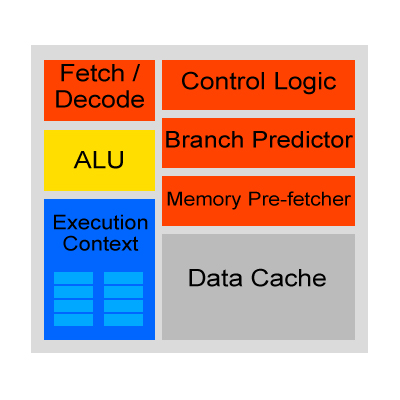
\includegraphics[width=.2\textwidth]{CPU-design.jpg} 
		\captionof{figure}{} 
\end{center}

\begin{center}
	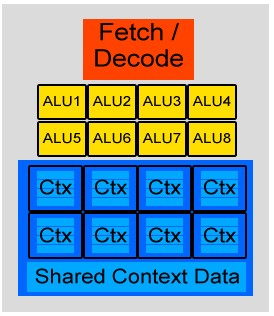
\includegraphics[width=.2\textwidth]{GPU-Design.jpg}
	\captionof{figure}{}
\end{center}





\begin{center}
		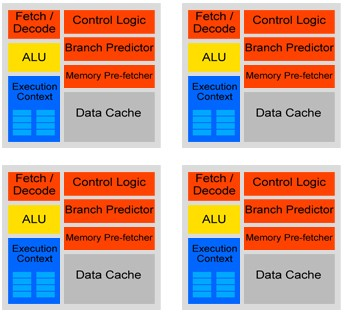
\includegraphics[width=.2\textwidth]{Multicore-CPU-design.jpg} 
		\captionof{figure}{} 
\end{center}

\begin{center}
	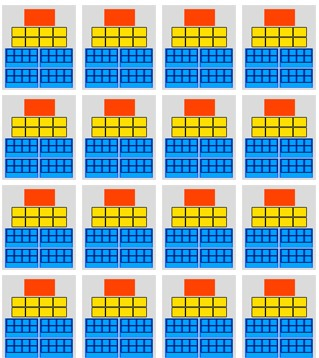
\includegraphics[width=.2\textwidth]{GPU-Design---multiple-cores.jpg}
	\captionof{figure}{}
\end{center}

\subsection{}

\section{Technical Sections}

\section{Simulation Methodology}

\section{Simulation Results}


\section{Conclusions}

\section{References}

\bibliographystyle{IEEEtran}
\bibliography{IEEEabrv,midterm}


% An example of a floating figure using the graphicx package.
% Note that \label must occur AFTER (or within) \caption.
% For figures, \caption should occur after the \includegraphics.
% Note that IEEEtran v1.7 and later has special internal code that
% is designed to preserve the operation of \label within \caption
% even when the captionsoff option is in effect. However, because
% of issues like this, it may be the safest practice to put all your
% \label just after \caption rather than within \caption{}.
%
% Reminder: the "draftcls" or "draftclsnofoot", not "draft", class
% option should be used if it is desired that the figures are to be
% displayed while in draft mode.
%
%\begin{figure}[!t]
%\centering
%\includegraphics[width=2.5in]{myfigure}
% where an .eps filename suffix will be assumed under latex, 
% and a .pdf suffix will be assumed for pdflatex; or what has been declared
% via \DeclareGraphicsExtensions.
%\caption{Simulation Results}
%\label{fig_sim}
%\end{figure}

% Note that IEEE typically puts floats only at the top, even when this
% results in a large percentage of a column being occupied by floats.


% An example of a double column floating figure using two subfigures.
% (The subfig.sty package must be loaded for this to work.)
% The subfigure \label commands are set within each subfloat command, the
% \label for the overall figure must come after \caption.
% \hfil must be used as a separator to get equal spacing.
% The subfigure.sty package works much the same way, except \subfigure is
% used instead of \subfloat.
%
%\begin{figure*}[!t]
%\centerline{\subfloat[Case I]\includegraphics[width=2.5in]{subfigcase1}%
%\label{fig_first_case}}
%\hfil
%\subfloat[Case II]{\includegraphics[width=2.5in]{subfigcase2}%
%\label{fig_second_case}}}
%\caption{Simulation results}
%\label{fig_sim}
%\end{figure*}
%
% Note that often IEEE papers with subfigures do not employ subfigure
% captions (using the optional argument to \subfloat), but instead will
% reference/describe all of them (a), (b), etc., within the main caption.


% An example of a floating table. Note that, for IEEE style tables, the 
% \caption command should come BEFORE the table. Table text will default to
% \footnotesize as IEEE normally uses this smaller font for tables.
% The \label must come after \caption as always.
%
%\begin{table}[!t]
%% increase table row spacing, adjust to taste
%\renewcommand{\arraystretch}{1.3}
% if using array.sty, it might be a good idea to tweak the value of
% \extrarowheight as needed to properly center the text within the cells
%\caption{An Example of a Table}
%\label{table_example}
%\centering
%% Some packages, such as MDW tools, offer better commands for making tables
%% than the plain LaTeX2e tabular which is used here.
%\begin{tabular}{|c||c|}
%\hline
%One & Two\\
%\hline
%Three & Four\\
%\hline
%\end{tabular}
%\end{table}


% Note that IEEE does not put floats in the very first column - or typically
% anywhere on the first page for that matter. Also, in-text middle ("here")
% positioning is not used. Most IEEE journals/conferences use top floats
% exclusively. Note that, LaTeX2e, unlike IEEE journals/conferences, places
% footnotes above bottom floats. This can be corrected via the \fnbelowfloat
% command of the stfloats package.


% trigger a \newpage just before the given reference
% number - used to balance the columns on the last page
% adjust value as needed - may need to be readjusted if
% the document is modified later
%\IEEEtriggeratref{8}
% The "triggered" command can be changed if desired:
%\IEEEtriggercmd{\enlargethispage{-5in}}

% references section

% can use a bibliography generated by BibTeX as a .bbl file
% BibTeX documentation can be easily obtained at:
% http://www.ctan.org/tex-archive/biblio/bibtex/contrib/doc/
% The IEEEtran BibTeX style support page is at:
% http://www.michaelshell.org/tex/ieeetran/bibtex/
%\bibliographystyle{IEEEtran}
% argument is your BibTeX string definitions and bibliography database(s)
%\bibliography{IEEEabrv,midterm.bib}
%
% <OR> manually copy in the resultant .bbl file
% set second argument of \begin to the number of references
% (used to reserve space for the reference number labels box)

%\begin{thebibliography}{1}

%\bibitem{IEEEhowto:kopka}
%H.~Kopka and P.~W. Daly, \emph{A Guide to \LaTeX}, 3rd~ed.\hskip 1em plus
%  0.5em minus 0.4em\relax Harlow, England: Addison-Wesley, 1999.

%\end{thebibliography}

%\bibliographystyle{ieeetr}
%\bibliography{midterm}

%\appendix
%\section{Project Progress}
%\subsection{Challenges Encountered}
%\subsection{Completed Tasks}
%\subsection{Remaining Tasks}


% that's all folks
%\bibliographystyle{ieeetr}
%\bibliography{midterm}




%\appendix
%\section{Project Progress}
%\subsection{Challenges Encountered}
%\subsection{Completed Tasks}
%\subsection{Remaining Tasks}

\end{document}


